\documentclass[aoas]{imsart}
%% LaTeX 2e style file for the processing of LaTeX2e files
%% of the following IMS/BS journals:
%%
%% - The Annals of Probability
%% - The Annals of Applied Probability
%% - The Annals of Statistics
%% - The Annals of Applied Statistics
%% - Statistical Science
%% - Probability Surveys
%% - Statistics Surveys
%% - Electronic Journal of Statistics
%% - Bernoulli
%% - Annales de l'Institut Henri Poincar\'e - Probabilit\'es et Statistiques
%% - Brazilian Journal of Probability and Statistics
%% - Bayesian Analysis
%%
%% - Institute of Mathematical Statistics, U.S.A.
%% - Bernoulli Society
%% - Institut Henry Poincare
%% - Brazilian Statistical Association
%% - International Society for Bayesian Analysis
%%
%% Macros written by Vytas Statulevicius, VTeX, Lithuania
%% Maintained by TeX group members, VTeX, Lithuania
%% for Institute of Mathematical Statistics, U.S.A.
%% Please submit bugs or your comments to latex-support@vtex.lt
%%
%% The original distribution is located at:
%% https://www.e-publications.org/ims/support

\RequirePackage{amsthm,amsmath,amsfonts,amssymb}
\RequirePackage[authoryear]{natbib}
\RequirePackage[colorlinks,citecolor=blue,urlcolor=blue]{hyperref}
\RequirePackage{graphicx}

% Added package
\usepackage[T1]{fontenc}
\usepackage[english]{babel}


% tightlist command for lists without linebreak
\providecommand{\tightlist}{%
  \setlength{\itemsep}{0pt}\setlength{\parskip}{0pt}}



% Garantees bookdown compilation
%\usepackage{lmodern}

\makeatletter
\def\maxwidth{\ifdim\Gin@nat@width>\linewidth\linewidth\else\Gin@nat@width\fi}
\def\maxheight{\ifdim\Gin@nat@height>\textheight\textheight\else\Gin@nat@height\fi}
\makeatother
% Scale images if necessary, so that they will not overflow the page
% margins by default, and it is still possible to overwrite the defaults
% using explicit options in \includegraphics[width, height, ...]{}
\setkeys{Gin}{width=\maxwidth,height=\maxheight,keepaspectratio}
% Set default figure placement to htbp
\makeatletter
\def\fps@figure{htbp}
\makeatother
\setlength{\emergencystretch}{3em} % prevent overfull lines

% alternative version to the shaded problem
\makeatletter
\@ifundefined{Shaded}{
}{\renewenvironment{Shaded}{\begin{kframe}}{\end{kframe}}}
\makeatother

\startlocaldefs
%%%%%%%%%%%%%%%%%%%%%%%%%%%%%%%%%%%%%%%%%%%%%
%                                          %%
% Uncomment next line to change            %%
% the type of equation numbering           %%
%                                          %%
%%%%%%%%%%%%%%%%%%%%%%%%%%%%%%%%%%%%%%%%%%%%%
\numberwithin{equation}{section}
%%%%%%%%%%%%%%%%%%%%%%%%%%%%%%%%%%%%%%%%%%%%%
%                                          %%
% For Axiom, Claim, Corollary, Hypothezis, %%
% Lemma, Theorem, Proposition              %%
% use \theoremstyle{plain}                 %%
%                                          %%
%%%%%%%%%%%%%%%%%%%%%%%%%%%%%%%%%%%%%%%%%%%%%
\theoremstyle{plain}
\newtheorem{axiom}{Axiom}
\newtheorem{claim}[axiom]{Claim}
\newtheorem{theorem}{Theorem}[section]
\newtheorem{lemma}[theorem]{Lemma}
%%%%%%%%%%%%%%%%%%%%%%%%%%%%%%%%%%%%%%%%%%%%%
%                                          %%
% For Assumption, Definition, Example,     %%
% Notation, Property, Remark, Fact         %%
% use \theoremstyle{remark}                %%
%                                          %%
%%%%%%%%%%%%%%%%%%%%%%%%%%%%%%%%%%%%%%%%%%%%%
\theoremstyle{remark}
\newtheorem{definition}[theorem]{Definition}
\newtheorem*{example}{Example}
\newtheorem*{fact}{Fact}
%%%%%%%%%%%%%%%%%%%%%%%%%%%%%%%%%%%%%%%%%%%%%
% Please put your definitions here:        %%
%%%%%%%%%%%%%%%%%%%%%%%%%%%%%%%%%%%%%%%%%%%%%
\endlocaldefs

% pandoc header
\usepackage{listings}
\usepackage{xcolor}
\usepackage{float}
\floatplacement{figure}{H}
% pandoc header
\usepackage{booktabs}
\usepackage{longtable}
\usepackage{array}
\usepackage{multirow}
\usepackage{wrapfig}
\usepackage{float}
\usepackage{colortbl}
\usepackage{pdflscape}
\usepackage{tabu}
\usepackage{threeparttable}
\usepackage{threeparttablex}
\usepackage[normalem]{ulem}
\usepackage{makecell}
\usepackage{xcolor}

\begin{document}



\begin{frontmatter}
%%%%%%%%%%%%%%%%%%%%%%%%%%%%%%%%%%%%%%%%%%%%%%
%%                                          %%
%% Enter the title of your article here     %%
%%                                          %%
%%%%%%%%%%%%%%%%%%%%%%%%%%%%%%%%%%%%%%%%%%%%%%
\title{STAT 444 FINAL PROJECT PROPOSAL}
%\title{A sample article title with some additional note\thanksref{T1}}
\runtitle{}
%\thankstext{T1}{A sample of additional note to the title.}



\begin{aug}
%%%%%%%%%%%%%%%%%%%%%%%%%%%%%%%%%%%%%%%%%%%%%%
%%Only one address is permitted per author. %%
%%Only division, organization and e-mail is %%
%%included in the address.                  %%
%%Additional information can be included in %%
%%the Acknowledgments section if necessary. %%
%%%%%%%%%%%%%%%%%%%%%%%%%%%%%%%%%%%%%%%%%%%%%%

%% Example:
%%\author[A]{\fnms{First} \snm{Author}\ead[label=e1]{first@somewhere.com}},
%%\author[B]{\fnms{Second} \snm{Author}\ead[label=e2,mark]{second@somewhere.com}}
%%\and
%%\author[B]{\fnms{Third} \snm{Author}\ead[label=e3,mark]{third@somewhere.com}}

\author[A]{\fnms{Angelo} \snm{Carreon}
  \ead[label=e1, mark]{jaccarre@uwaterloo.ca}}
  ,
\author[A]{\fnms{Hoseok} \snm{Lee}
  \ead[label=e2, mark]{h349lee@uwaterloo.ca}}
  
\author[A]{\fnms{Joy} \snm{Chen}
  \ead[label=e3, mark]{z635chen@uwaterloo.ca}}
  and
\author[A]{\fnms{Steven} \snm{Shen}
  \ead[label=e4, mark]{s58shen@uwaterloo.ca}}
  

%%%%%%%%%%%%%%%%%%%%%%%%%%%%%%%%%%%%%%%%%%%%%%
%% Addresses                                %%
%%%%%%%%%%%%%%%%%%%%%%%%%%%%%%%%%%%%%%%%%%%%%%
%% Example:
%%\address[B]{Department,
%%University or Company Name,
%%\printead{e2,e3}}
\address[A]{Department of Statistics and Actuarial Science, University
of Waterloo,
  \printead{e1,e2,e3,e4}}
\end{aug}

\begin{abstract}
This paper contains our proposal for the STAT 444 final project. It
outlines our dataset, performs some brief exploratory data analysis,
then outlines our approach to fitting regression models to predict a
final sale price of a house given its physical attributes.
\end{abstract}


\begin{keyword}
\kwd{housing}
\kwd{advanced regression}
\end{keyword}

\end{frontmatter}


\newenvironment{kframe}{}{}

\hypertarget{introduction-to-our-chosen-dataset}{%
\section{Introduction to our chosen
dataset}\label{introduction-to-our-chosen-dataset}}

Our project aims to assess the feasibility of utilizing regression
techniques for interpolating and modeling housing prices. We have
selected a dataset of housing prices in Ames, Iowa, along with their
features from the \emph{Journal of Statistics Education}
\citep{cock2011amesdataset}. This dataset was prepared by Dean De Cock
for use as an end-of-semester regression project. His intent was to
provide data of substantial size (\(n=2930\)) with easy-to-understand
variables that are known to affect the final sale price such as build
date, lot size, and living space square footage. Applying this to
today's real estate market, we wish to answer the following question:
\emph{which regression method best predicts the prices of houses given
their characteristics}?

\hypertarget{exploratory-data-analysis}{%
\section{Exploratory Data Analysis}\label{exploratory-data-analysis}}

This dataset contains 2930 rows and 82 columns. There are 80 explanatory
variables, consisting of 23 nominal, 23 ordinal, 14 discrete, and 20
continuous variables. Several columns contain many missing values and
will be dropped before we begin fitting models. As highlighted in De
Cock's paper, several unusual outlier house sales exist in the data;
these will also be removed. There are no duplicate rows.

As seen in table \ref{resp}, the distribution of \texttt{Sale\ Price} is
significantly right-skewed. The sale prices range from \$12,789 to
\$755,000 with a mean of \$180,796 and a standard deviation of
\$79,886.69. To achieve a more normal distribution, we can apply a log
transformation on the dependent variable, as seen below:

\begin{figure}
\centering
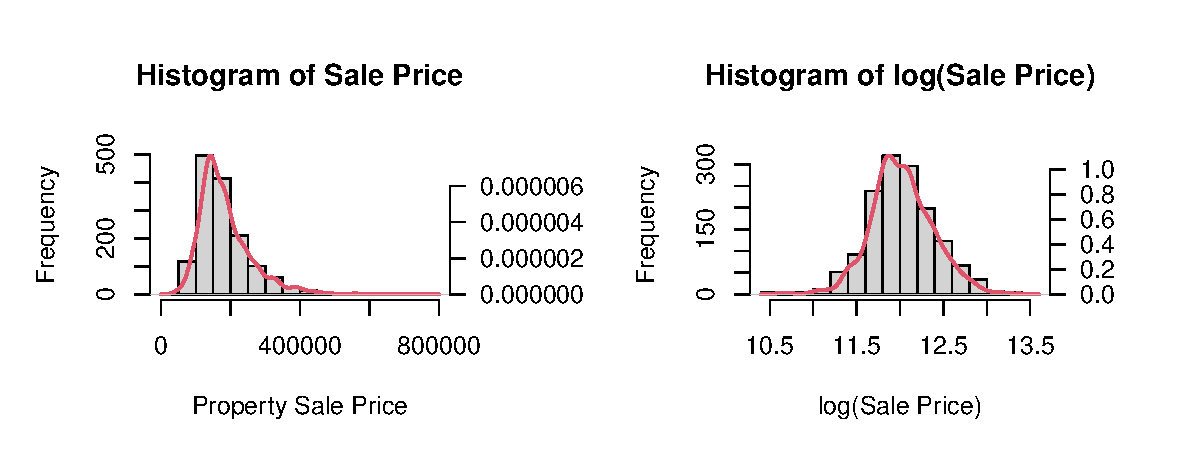
\includegraphics{STAT-444-FINAL-PROJECT-PROPOSAL_files/figure-latex/unnamed-chunk-3-1.pdf}
\caption{Histograms of the response variable, Sale Price\label{resp}}
\end{figure}

Some variables of interest are \texttt{Neighbourhood} and
\texttt{LotArea}, where we see in table \ref{neighbourhood} to have
significant differences in the average property sale price. One way in
which these neighborhoods could differ is in the size of the lots of the
houses that reside there. Our team would need to consider variable
associations such as these to deal with collinearity.

\begin{figure}
\centering
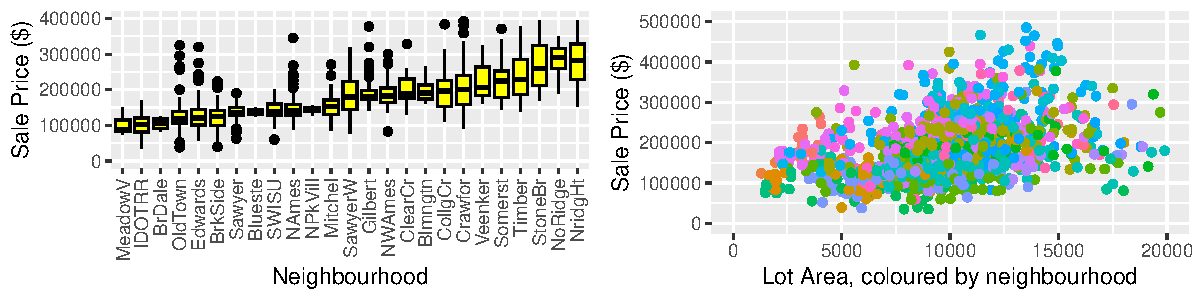
\includegraphics{STAT-444-FINAL-PROJECT-PROPOSAL_files/figure-latex/unnamed-chunk-4-1.pdf}
\caption{Plots showing the distribution of final Sale Price across the
different Neighborhoods\label{neighbourhood}}
\end{figure}

\hypertarget{plan}{%
\section{Plan}\label{plan}}

The objective of this study is to determine the viability and
effectiveness of employing additive models, splines, and polynomial
regression for predicting house prices. We focus our attention on the
following:

\begin{itemize}
\item
  \textbf{Accuracy}: Assess the predictive accuracy of additive models,
  splines, and polynomial regression in comparison to traditional
  regression models commonly used in the real estate domain.
    \vspace{0.2cm}
\item
  \textbf{Flexibility}: Analyze the ability of these techniques to
  capture complex relationships between house price predictors, such as
  square footage, location, number of bedrooms, and other relevant
  features.
  \vspace{0.2cm}
\item
  \textbf{Interpretability}: Evaluate the interpretability and
  explainability of the models, ensuring that the predictions can be
  easily understood and justified by stakeholders.
  \vspace{0.2cm}
\end{itemize}

To achieve our objective, we propose the following methodology as an
outline:

\begin{enumerate}
\item
  \textbf{Initial Benchmark}: Use the performance of linear regression, with simple categorical encoding, on the full
  feature set as an initial benchmark.
  \vspace{0.2cm}
\item
  \textbf{Data Preprocessing}: Handle missing/invalid values and outliers and perform feature engineering to enhance
  the models' predictions. To mitigate the "curse of dimensionality" and reduce collinearity in the dataset, we
   will use a low variance filter and clustering techniques such as Principal Component Analysis (PCA).
   \vspace{0.2cm}
\item
  \textbf{Model Implementation}: Develop additive models, splines, and
  polynomial regression models using appropriate algorithms and
  frameworks, such as generalized additive models (GAMs) and polynomial
  regression libraries in R. We will also apply penalization techniques
  to prevent overfitting (e.g. forward/backward selection, LASSO/Ridge regression)
  while including interactions between covariates to model any non-linear relationships.
  \vspace{0.2cm}
\item
  \textbf{Model Evaluation}: Assess the performance of the models using
  appropriate evaluation metrics, such as mean squared error (MSE), root
  mean squared error (RMSE), and R-squared values and compare the
  results with benchmark models.
  \vspace{0.2cm}
\item
  \textbf{Interpretation and Explainability}: Examine the contributions of each
  feature and the underlying relationships identified by the models. Visualize the results in an intuitive yet
  comprehensive manner.
\end{enumerate}

\bibliographystyle{imsart-nameyear}
\bibliography{ims.bib}


\end{document}
